% factorisation types of two quintics mod p<1e5 vs class proportions (generated by a script).
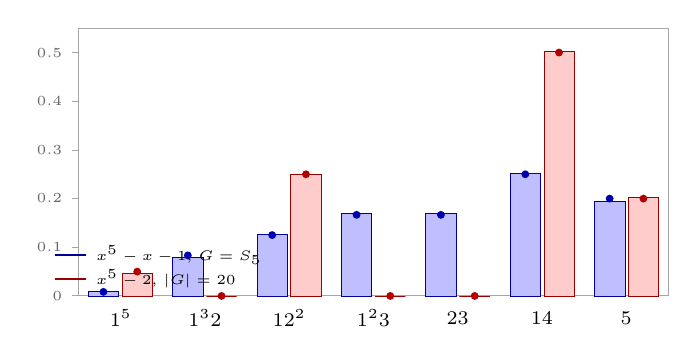
\begin{tikzpicture}[x=1cm,y=1cm]
\draw[black!35] (0,0) rectangle (7.50,3.40);
\draw[black!35] (0,0.00)--(-0.08,0.00) node[left,font=\tiny,black!60]{$0$};
\draw[black!35] (0,0.62)--(-0.08,0.62) node[left,font=\tiny,black!60]{$0.1$};
\draw[black!35] (0,1.24)--(-0.08,1.24) node[left,font=\tiny,black!60]{$0.2$};
\draw[black!35] (0,1.85)--(-0.08,1.85) node[left,font=\tiny,black!60]{$0.3$};
\draw[black!35] (0,2.47)--(-0.08,2.47) node[left,font=\tiny,black!60]{$0.4$};
\draw[black!35] (0,3.09)--(-0.08,3.09) node[left,font=\tiny,black!60]{$0.5$};
\node[font=\scriptsize] at (0.54,-0.28) {$1^5$};
\node[font=\scriptsize] at (1.61,-0.28) {$1^32$};
\node[font=\scriptsize] at (2.68,-0.28) {$12^2$};
\node[font=\scriptsize] at (3.75,-0.28) {$1^23$};
\node[font=\scriptsize] at (4.82,-0.28) {$23$};
\node[font=\scriptsize] at (5.89,-0.28) {$14$};
\node[font=\scriptsize] at (6.96,-0.28) {$5$};
\filldraw[blue!25,draw=blue!60!black,line width=0.2pt] (0.129,0) rectangle (0.514,0.053);
\filldraw[blue!25,draw=blue!60!black,line width=0.2pt] (1.200,0) rectangle (1.586,0.497);
\filldraw[blue!25,draw=blue!60!black,line width=0.2pt] (2.271,0) rectangle (2.657,0.777);
\filldraw[blue!25,draw=blue!60!black,line width=0.2pt] (3.343,0) rectangle (3.729,1.044);
\filldraw[blue!25,draw=blue!60!black,line width=0.2pt] (4.414,0) rectangle (4.800,1.054);
\filldraw[blue!25,draw=blue!60!black,line width=0.2pt] (5.486,0) rectangle (5.871,1.553);
\filldraw[blue!25,draw=blue!60!black,line width=0.2pt] (6.557,0) rectangle (6.943,1.205);
\filldraw[red!20,draw=red!60!black,line width=0.2pt] (0.557,0) rectangle (0.943,0.290);
\filldraw[red!20,draw=red!60!black,line width=0.2pt] (1.629,0) rectangle (2.014,0.000);
\filldraw[red!20,draw=red!60!black,line width=0.2pt] (2.700,0) rectangle (3.086,1.541);
\filldraw[red!20,draw=red!60!black,line width=0.2pt] (3.771,0) rectangle (4.157,0.000);
\filldraw[red!20,draw=red!60!black,line width=0.2pt] (4.843,0) rectangle (5.229,0.000);
\filldraw[red!20,draw=red!60!black,line width=0.2pt] (5.914,0) rectangle (6.300,3.102);
\filldraw[red!20,draw=red!60!black,line width=0.2pt] (6.986,0) rectangle (7.371,1.249);
\fill[blue!70!black] (0.321,0.052) circle (0.05cm);
\fill[blue!70!black] (1.393,0.515) circle (0.05cm);
\fill[blue!70!black] (2.464,0.773) circle (0.05cm);
\fill[blue!70!black] (3.536,1.030) circle (0.05cm);
\fill[blue!70!black] (4.607,1.030) circle (0.05cm);
\fill[blue!70!black] (5.679,1.545) circle (0.05cm);
\fill[blue!70!black] (6.750,1.236) circle (0.05cm);
\fill[red!70!black] (0.750,0.309) circle (0.05cm);
\fill[red!70!black] (1.821,0.000) circle (0.05cm);
\fill[red!70!black] (2.893,1.545) circle (0.05cm);
\fill[red!70!black] (3.964,0.000) circle (0.05cm);
\fill[red!70!black] (5.036,0.000) circle (0.05cm);
\fill[red!70!black] (6.107,3.091) circle (0.05cm);
\fill[red!70!black] (7.179,1.236) circle (0.05cm);
\draw[blue!60!black,thick] (-0.30,0.52)--(0.10,0.52) node[right,font=\tiny,black]{$x^5-x-1$, $G=S_5$};
\draw[red!60!black,thick] (-0.30,0.22)--(0.10,0.22) node[right,font=\tiny,black]{$x^5-2$, $|G|=20$};
\end{tikzpicture}
